\section{Experimentacion y resultados}

Para analizar los algortimos implementados vamos a utilizar varios archivos de test generados por nosotros, los cuales estan mas detallados en el apendice, con el fin de realizar una serie de test que nos permitirán en primer caso encontrar parametros buenos con lo que ejecutar los distintos metodos y posteriormente evaluar el desempeño de la implementación mediante las métricas propuestas por la cátedra.

Dividimos la experimentación en dos secciones, una para cada archivo de prueba. Y evaluaremos los parametros individualmente para cada una de ellas

\subsection {Algoritmo de K-NN}

Lo primero que vamos a hacer es encontrar un valor de $K$ que nos permita maximizar la cantidad de aciertos, sin tener en consideración las métricas.

Ejecutamos el algoritmos de $K-NN$ variando los valores de k entre {1..30} dejando fija la cantidad de particiones para $K=$6 y $K=$15. Luego para cada una de las iteraciones tomamos el promedio, esto se utilizo tanto para la cantidad de aciertos como para la cantidad de vecinos.

Cada uno de los conjuntos conto con 4200 imagenes a testear. En los siguientes graficos presentamos algunos de los sets obtenidos:

Expresamos los aciertos para cada K en con el siguiente gráfico:
\begin{center}
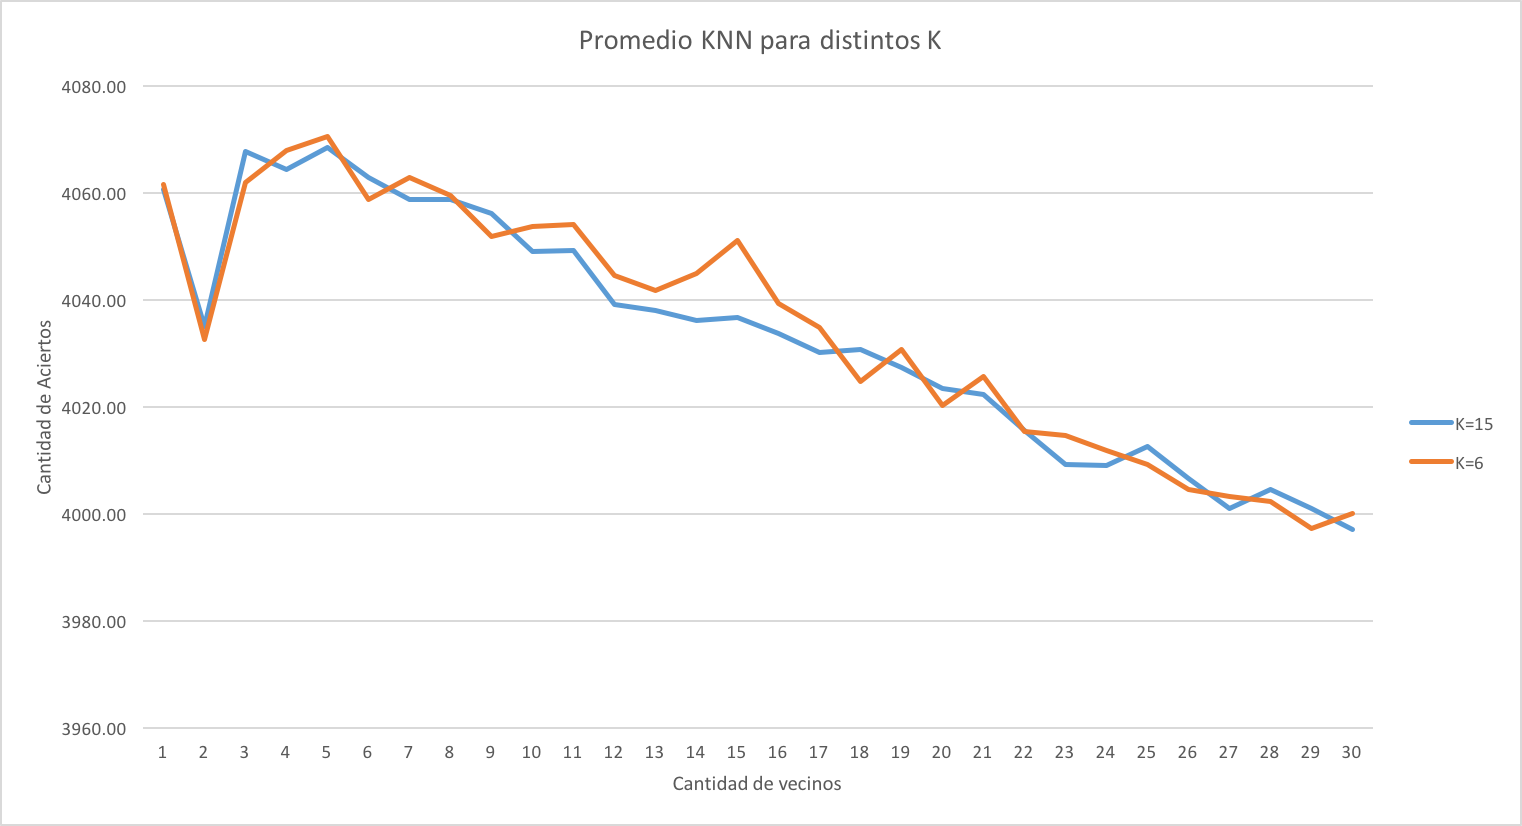
\includegraphics[scale=0.6]{imagenes/AciertosKNN.png}
\end{center}

Como se puede observar para ambos $K$ tienen el mismo patron a lo largo que se incrementa la cantidad de vecinos $k$, pero ambas parecen alcanzar un maximo en $k=5$ como cantidad de vecinos. Además notemos que a medida que se incrementa el valor de $k$ la cantidad de aciertos va disminuyendo levemente, cumpliendo lo mencionado en el desarrollo. Cuanto mas corta sea la distancia de los vecinos, mas chances hay de tener un acierto sin importar el valor de $K$.

Si nos detenemos y obsvervamos con mas claridad cuando para la combinacion de $K$=6 y $k$=5 es donde se maximizan en comparativa para knn, lo que intentaremos hacer en los proximos metodos es utilizar esta convinacion de $K$=6 y ir variando la cantidad de vecinos mas cercanos para ver si existe algun tipo de relacion con el fin de asegurar que esa convinacion es la mejor.

Por otro lado hicimos un analisis temporal para saber como afectaba la cantidad de particiones que tomamos para el cross validation y variamos la cantidad de vecinos tomados para ver como se comportaba, los cuales arrojaron los siguientes resultados. 

\begin{center}
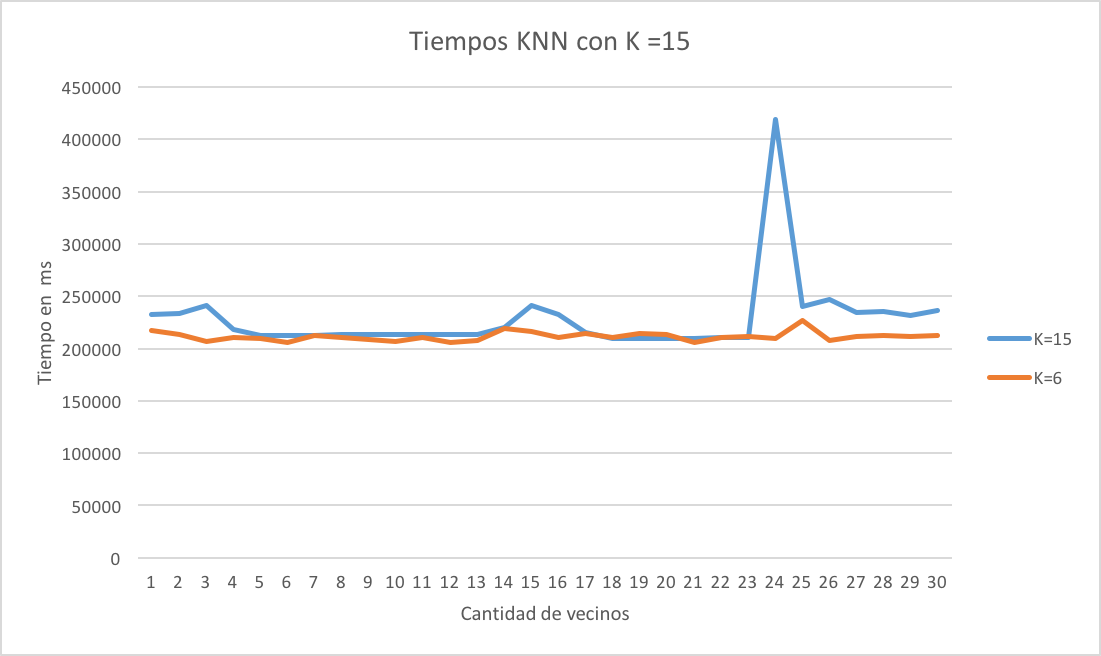
\includegraphics[scale=0.6]{imagenes/TiemposKNN.png}
\end{center}

En cuanto a los tiempos para diferentes $K$ no varian mucho en la media, si bien se puede notar al principio que a mayor cantidad de ejecuciones mayor es el tiempo que demora, algo prevesible previamente. Lo que notamos es que hay un pico cuando tomamos entre 23 y 25 vecinos mas cercanos.Sin embargo,esto es un caso que deberiamos seguir ejecutando para esos parametros con el fin de ver si no es ruido que se pudo haber generado por otro proceso en el momento de la ejecucion para descartar esto.


\subsection {Algoritmo de K-NN con Optimización de PCA}
Para el algoritmo de PCA lo que realizamos fue una variacion de los valores de lambda (cantidad de componentes principales) en el algoritmo de pca. Para esos valores de $K$ medimos los tiempos de ejecución y los promediamos para poder ver de que manera varía la ejecución de los algoritmos en función de $\alpha$, luego tomamos un promedio de las ejecuciones y obtuvimos lo siguientes resultados:

\begin{center}
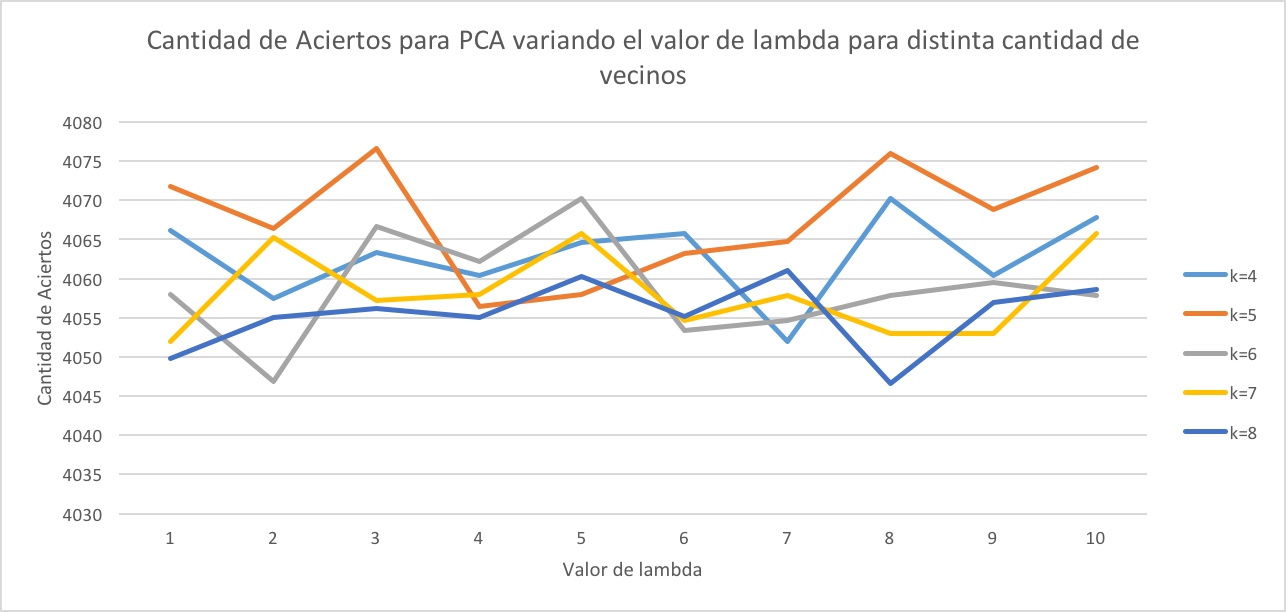
\includegraphics[scale=0.6]{imagenes/AciertosPCA.png}
\end{center}

Al ver estos resultados notamos a comparacion de los resultados obtenidos para KNN con $k$=5 se respetan para la optimizacion, ya que mirando las comvinaciones de lambda con cantidad de vecinos el que resulta como 'ganador' arrojando una cantidad de aciertos mayor a 4075 es cuando $k$=5 y $\lambda$=3. 

A medida crecia el lamda no parece llegar a igualarlo pero si esta muy cerca cuando se toman 8 componentes principales. 

\begin{center}
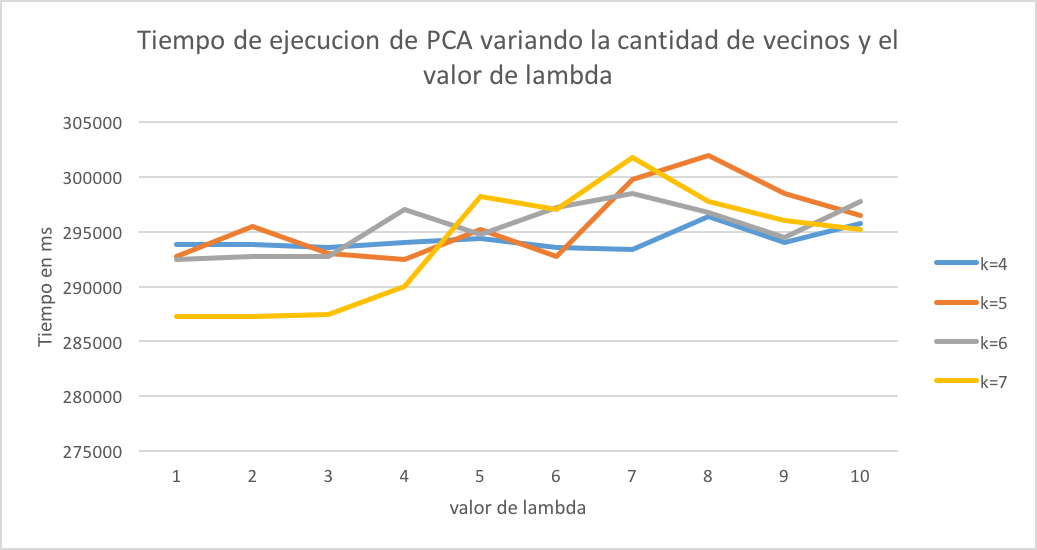
\includegraphics[scale=0.6]{imagenes/TiemposPCA.png}
\end{center}

En cuanto a los tiempos podemos cabe aclarar que estos tiempos no contemplan todo lo que se considera el ’entrenamiento’ del sistema, es decir, todo el preprocesamiento que resultara en encontrar
los valores principales. La justificacion de esto es que el procedimiento se realizar ́a una vez, para entrenar el sistema y luego, al momento de clasificar las
nuevas imagenes este tiempo podra ser despreciado.Este grafico se puede ver que aumentar el α produce un aumento lineal de los tiempos de ejecucion, 
de lo que se desprende que aumentar la cantidad valores principales no resulta gratuito en terminos de tiempo de ejecucion y tiene cierto costo asociado.

De igual manera la distribucion de tiempos al variar el lamda parece ir creciendo levemente y podriamos predecir que asi va a hacer mientras mas grande sea el valor de lambda.

\subsection {Algoritmo de K-NN con Optimización de PSL-DA}
Habiendo fijado k = 3 , corremos el test1.in variando el gamma utilizando los valores 1,2,10 y 50. Aqui el grafico
\begin{figure}[H]
\centering
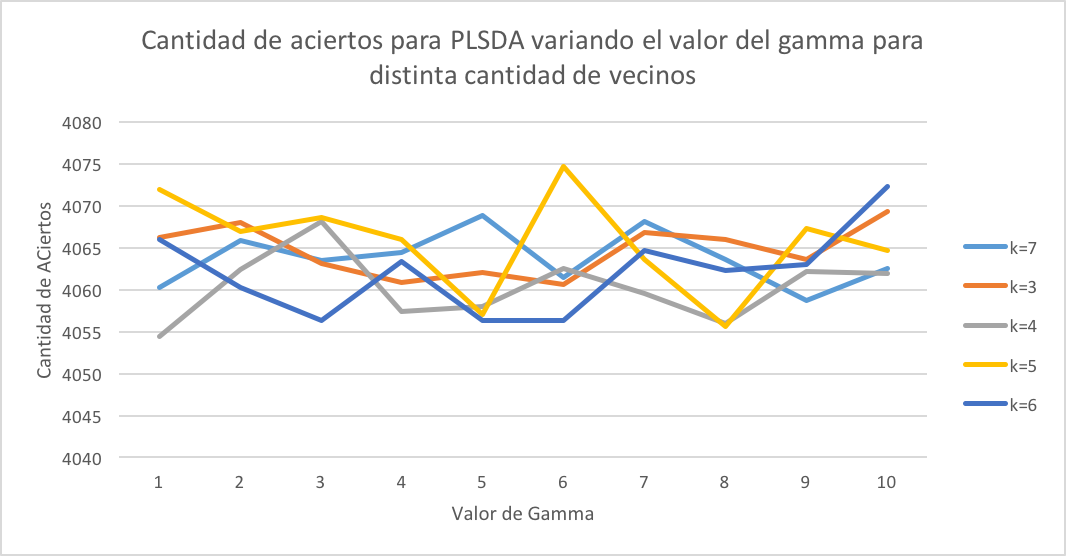
\includegraphics[width=1\textwidth]{imagenes/AciertosPLSDA.png}
\caption{Comparacion de aciertos variando el gamma}
\label{fig:Comparacion de tecnicas}
\end{figure}


\begin{center}
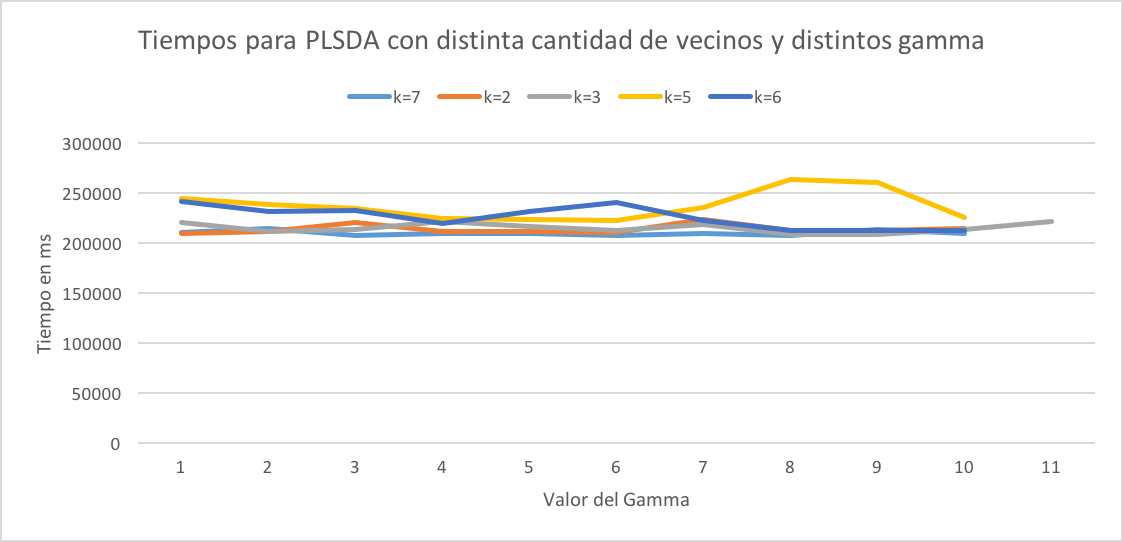
\includegraphics[scale=0.6]{imagenes/TiemposPLSDA.png}
\end{center}

Vemos que si aumenta el gamma , mejora la precision pero si gamma aumenta demasiado , en algun momento empeora tu hit rate , suponemos que eso se debe a que si bien tenemos bastante informacion , la cantidad de vecinos no permite aprovecharla . Eso hace suponer que para que tengamos un buen hit rate , debe haber algun tipo de relacion entre el k y el gamma . Eso se va a poner a prueba usando el test2.in

\subsection {Algoritmo de K-NN con Optimización de PSL-DA}



